\subsection{Ascape}

Ascape 这款应用通过 360° 无缝全景视频让你通过景色的立体画面切身体验视频中呈现的著名景点,探索只有当地人才知道的隐藏宝藏的经历。并且镜头会伴随着你的移动,画面的位置和显示的角度都会随之改变,见图\ref{fig:ascape1}。

\begin{figure}[htp]
\centering
\fbox{
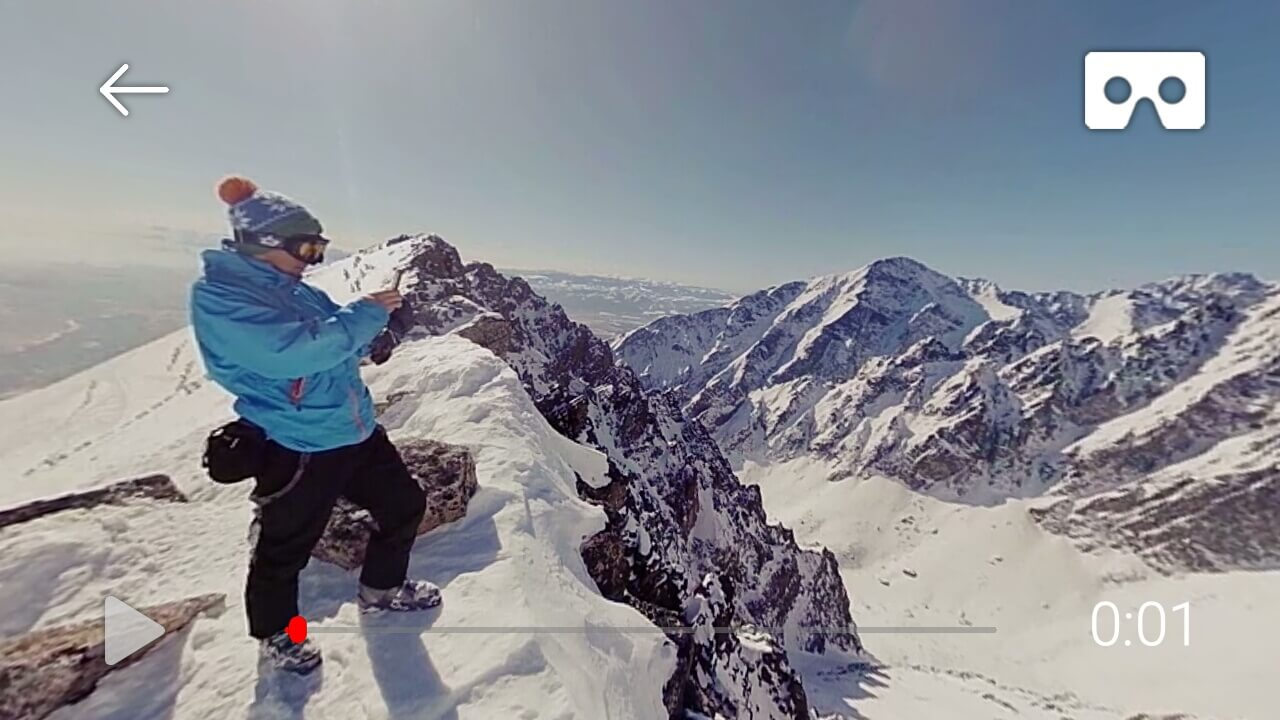
\includegraphics[width=.7\textwidth]{ascape2}
}
\caption{简洁的全景视频播放}
\label{fig:ascape1}
\end{figure}

同时,这款应用在 APP 传统界面上也继承了欧美一向以来的简约风格:“探索”页面采用卡片设计模式直观展示了新奇的场景;“发现”页面通过地图和名单两种模式展示了全球各地的场景选项;“我的旅行”也通过卡片模式展示了已下载的全景场景,见图\ref{fig:ascape2}。

\begin{figure}[htp]
\centering
\fbox{
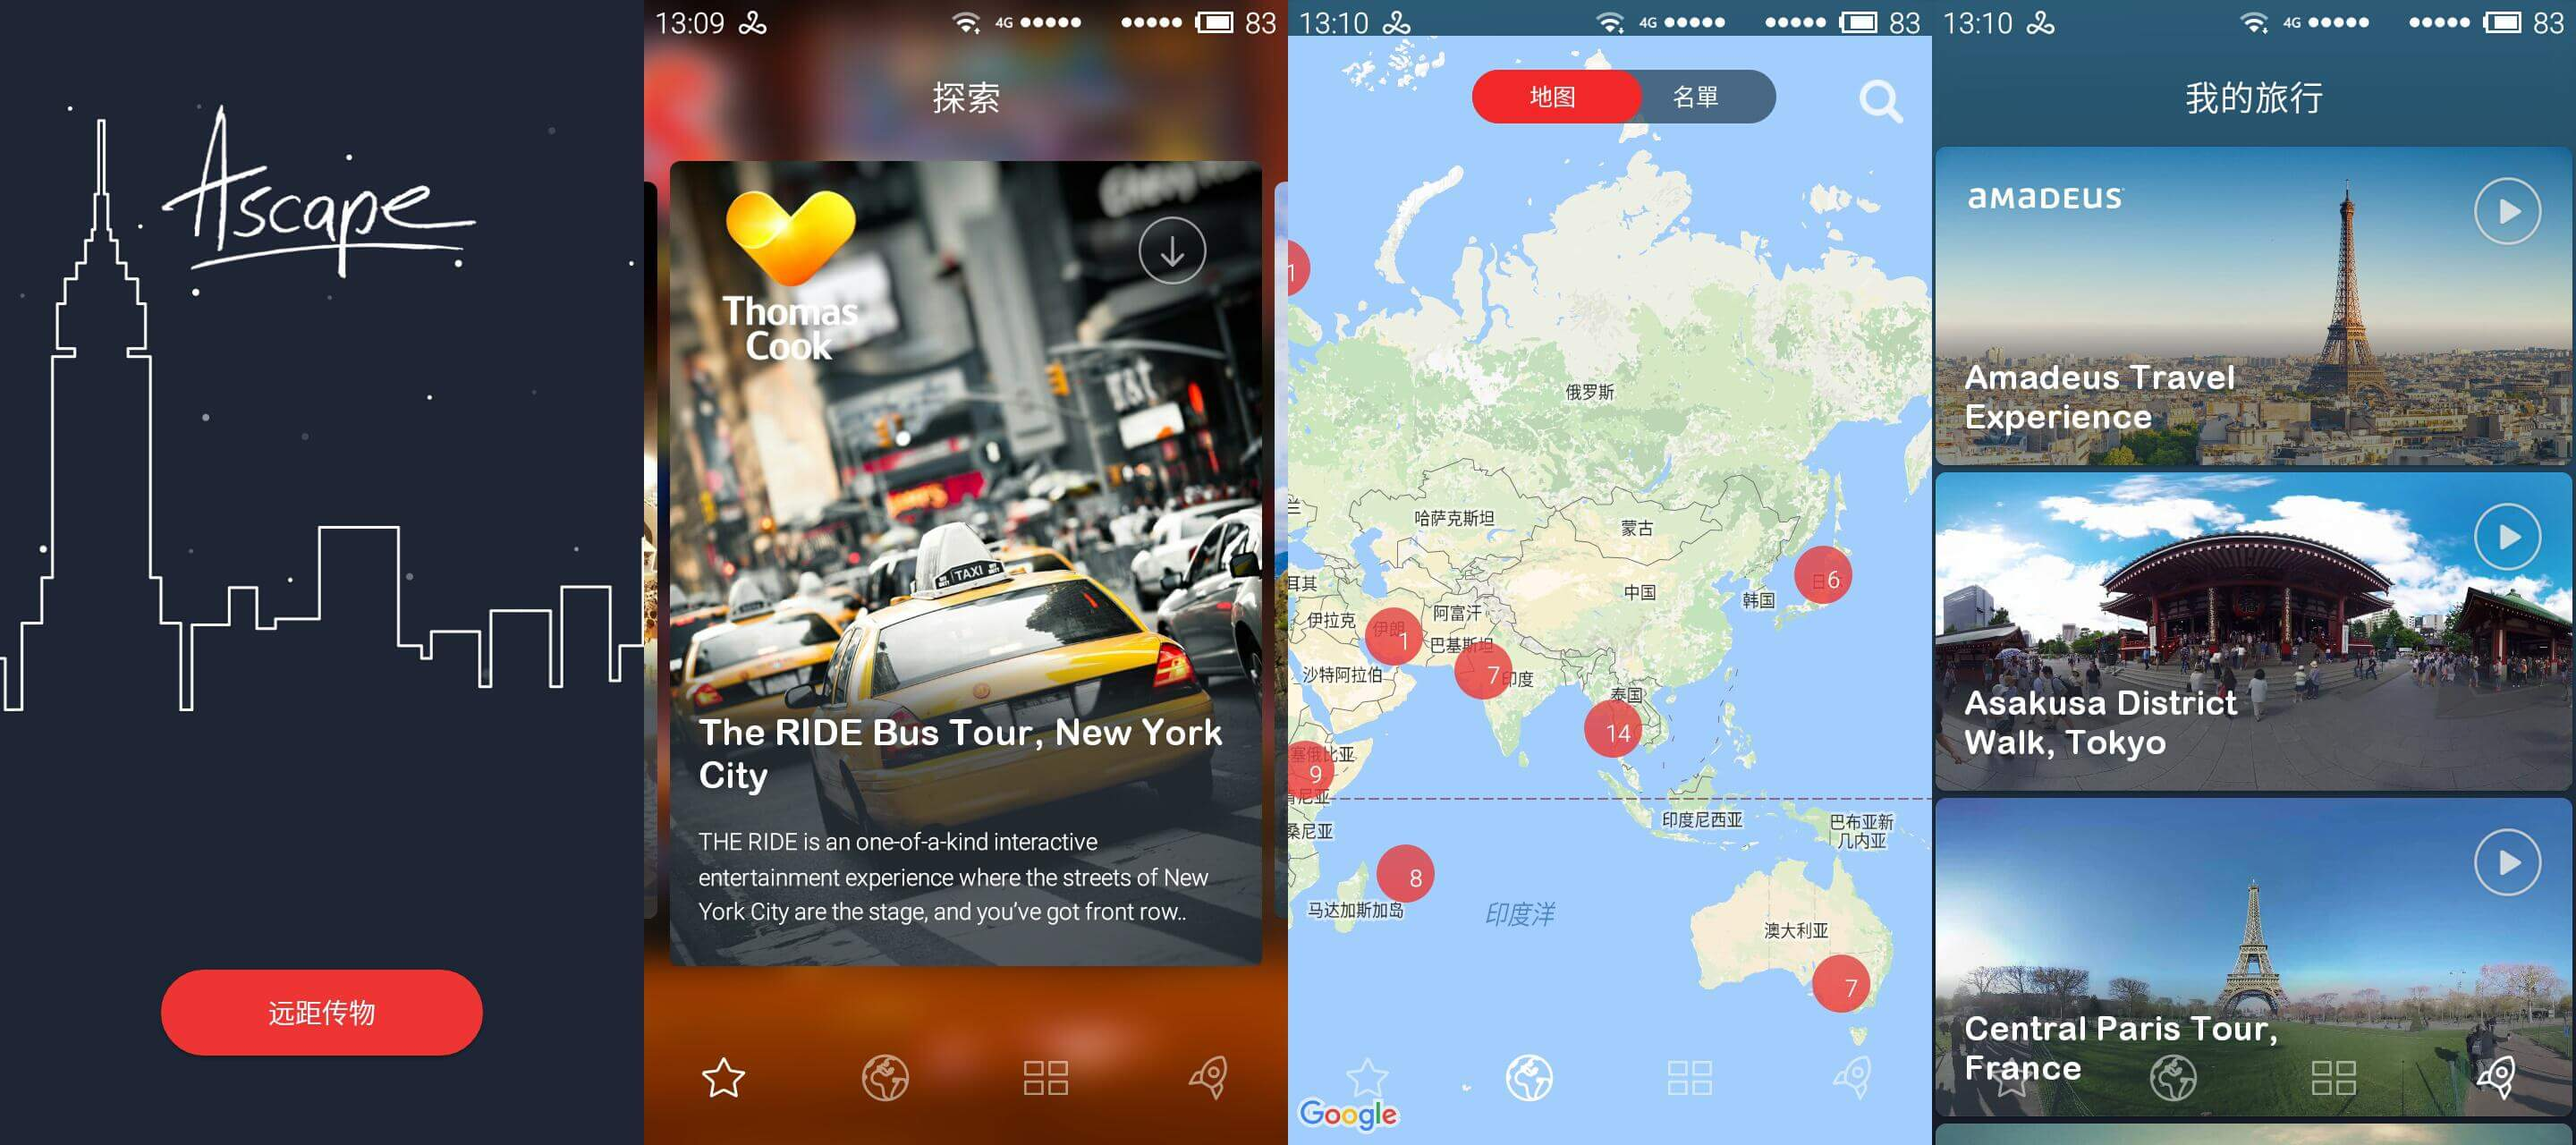
\includegraphics[width=.7\textwidth]{ascape1}
}
\caption{简洁的全景视频播放}
\label{fig:ascape2}
\end{figure}

\subsection{Fulldive}

Fulldive 是一个智能手机与虚拟场景连接的平台,进入 APP 后即进入了一个全景漫游的世界。场景内包含常用的网络视频、本地视频/图片、VR 相机、VR 浏览器等应用,同时支持从其内部市场下载更多基于其开发的 VR 应用,见图\ref{fig:fulldive1}。

\begin{figure}[htp]
\centering
\fbox{
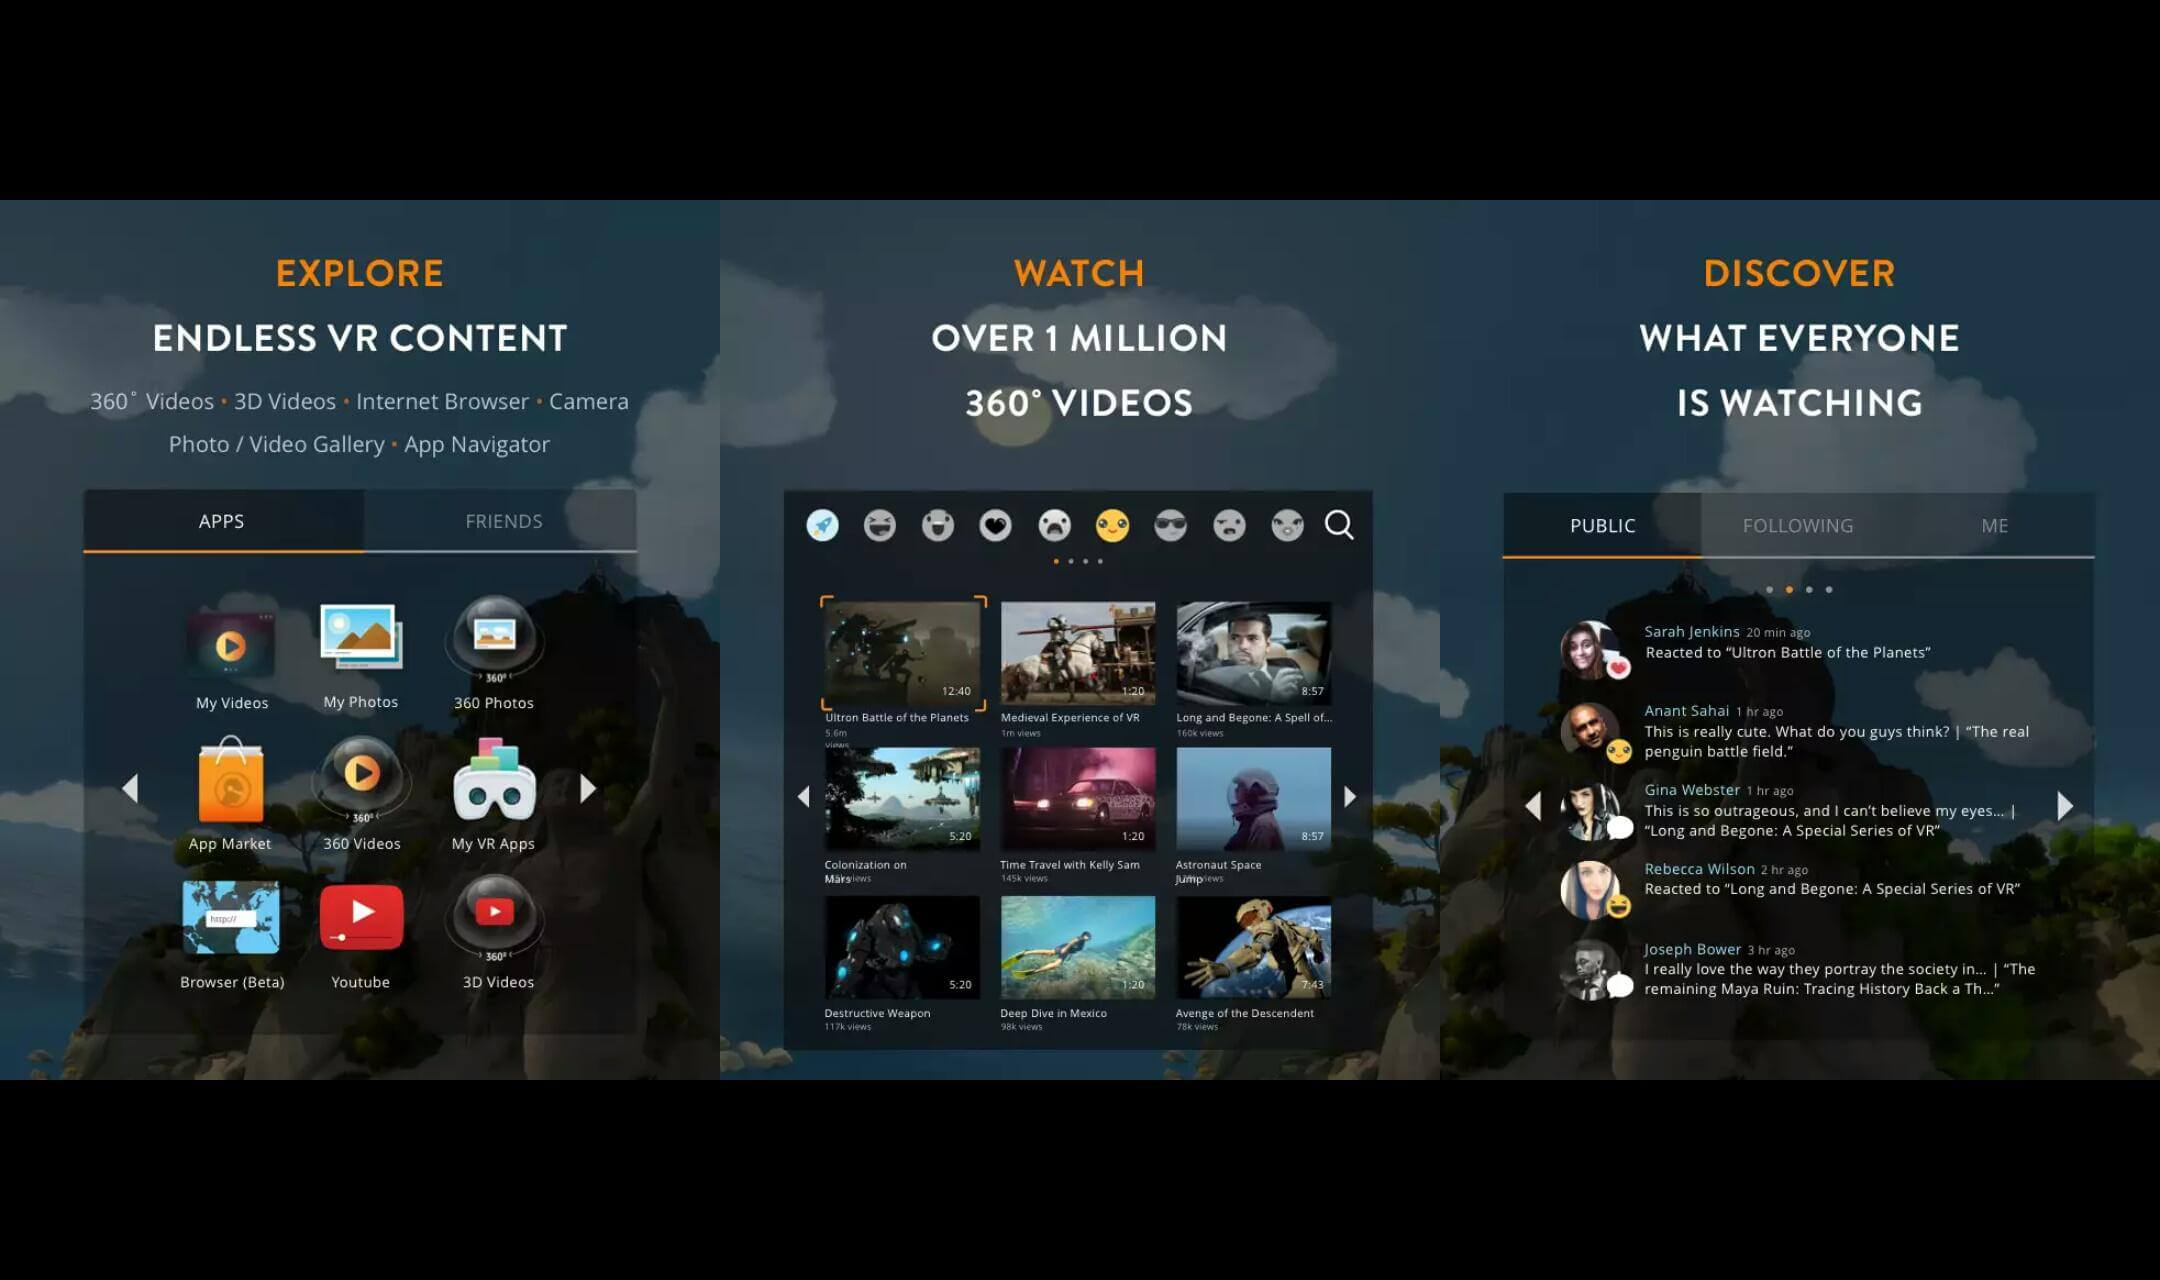
\includegraphics[width=.7\textwidth]{fulldive1}
}
\caption{Fulldive 内置的应用列表}
\label{fig:fulldive1}
\end{figure}

与 Ascape 不同之处在于 Fulldive 的操控完全是在虚拟全景中,所以在播放视频及操作选项时 Fulldive 有一些针对配戴 VR 眼镜者所特别提供的操作方式,见图\ref{fig:fulldive2}。例如,将视线聚焦在某个按钮上超过 3 秒后即视为按下了该按钮。这是一种与桌面鼠标和触屏点按都完全不同的交互形式,借鉴了鼠标的双击或是触屏的长按这两种操作,见图\ref{fig:fulldive3}。

\begin{figure}[htp]
\centering
\fbox{
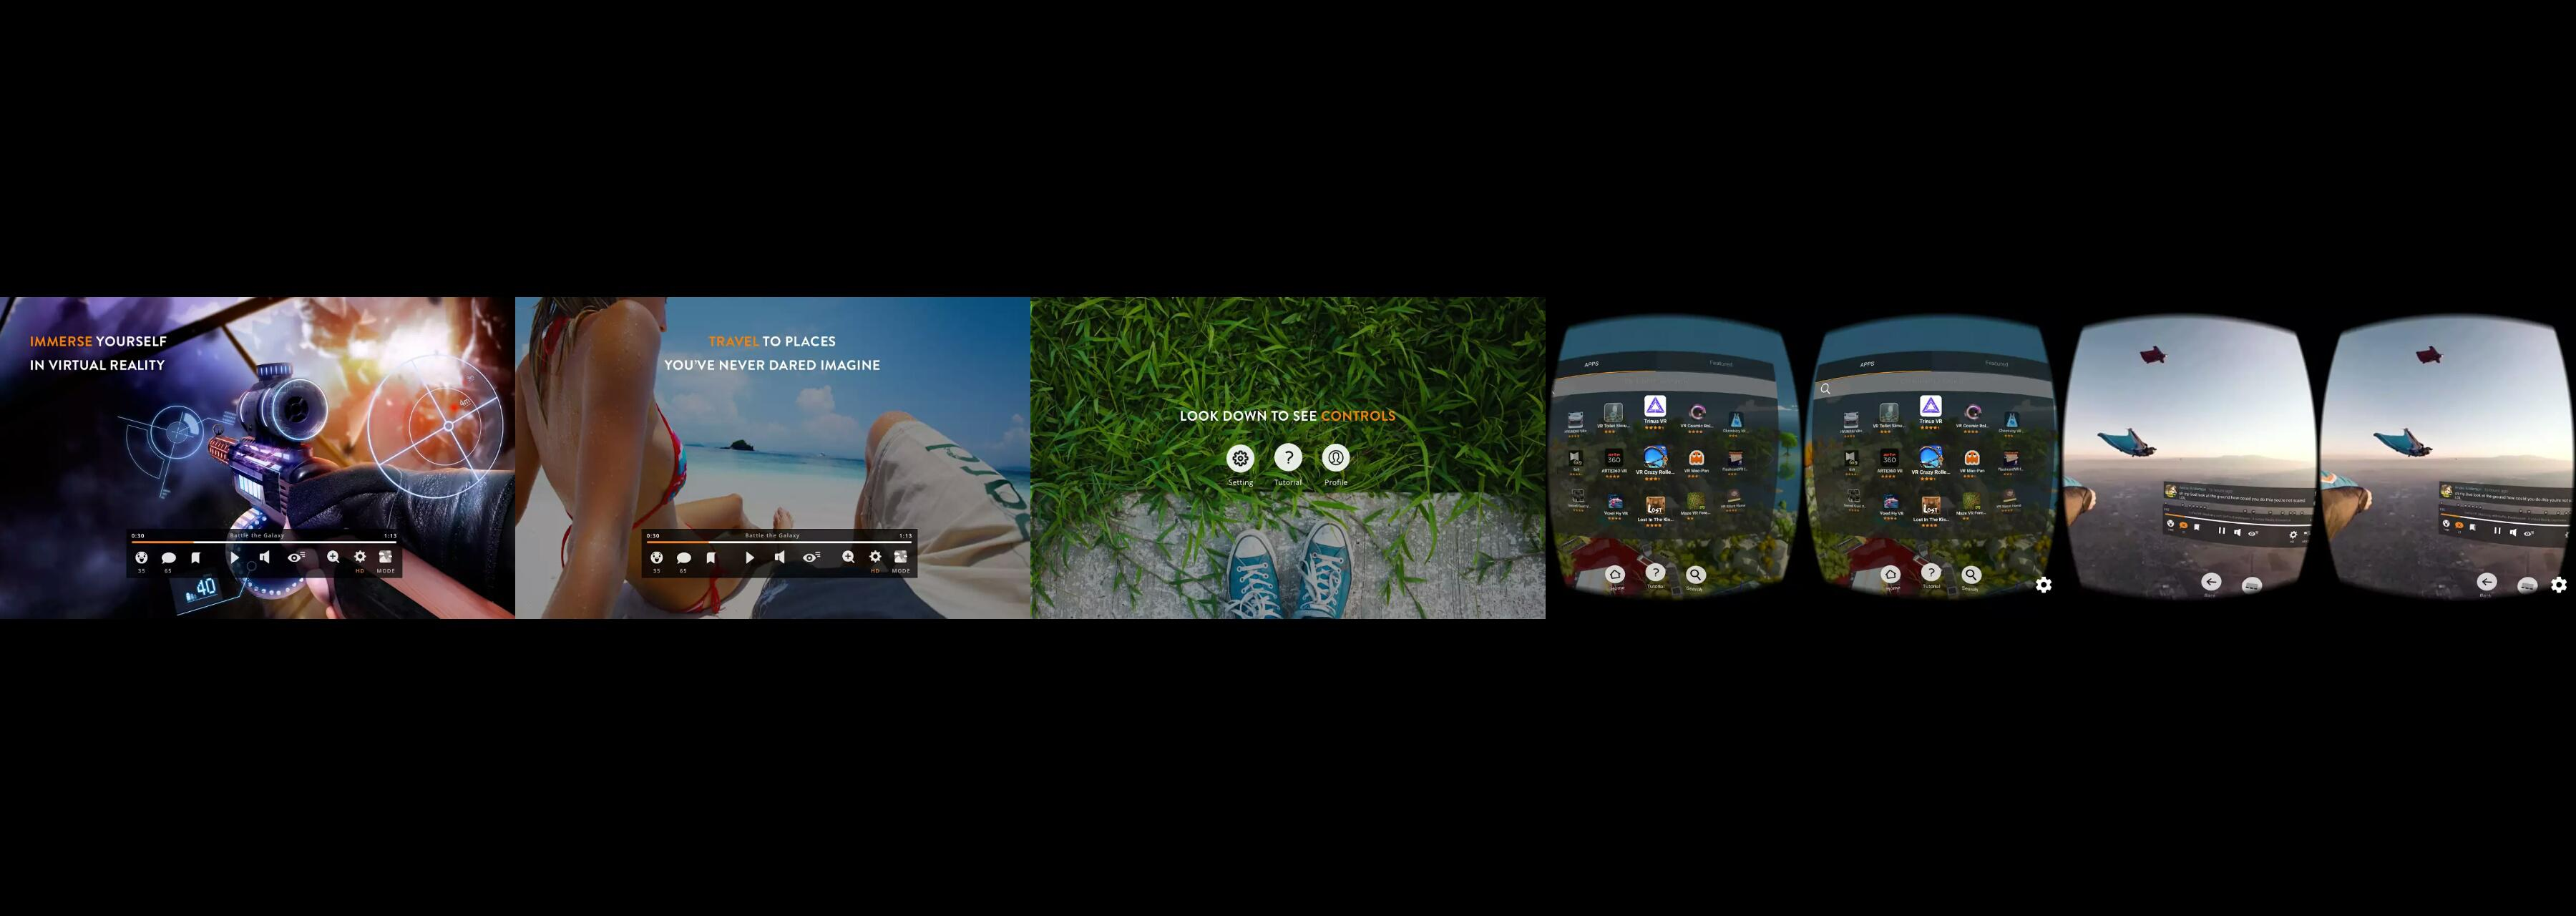
\includegraphics[width=.6\textwidth]{fulldive2}
}
\caption{Fulldive 特有操作形式}
\label{fig:fulldive2}
\end{figure}

\begin{figure}[htp]
\centering
\fbox{
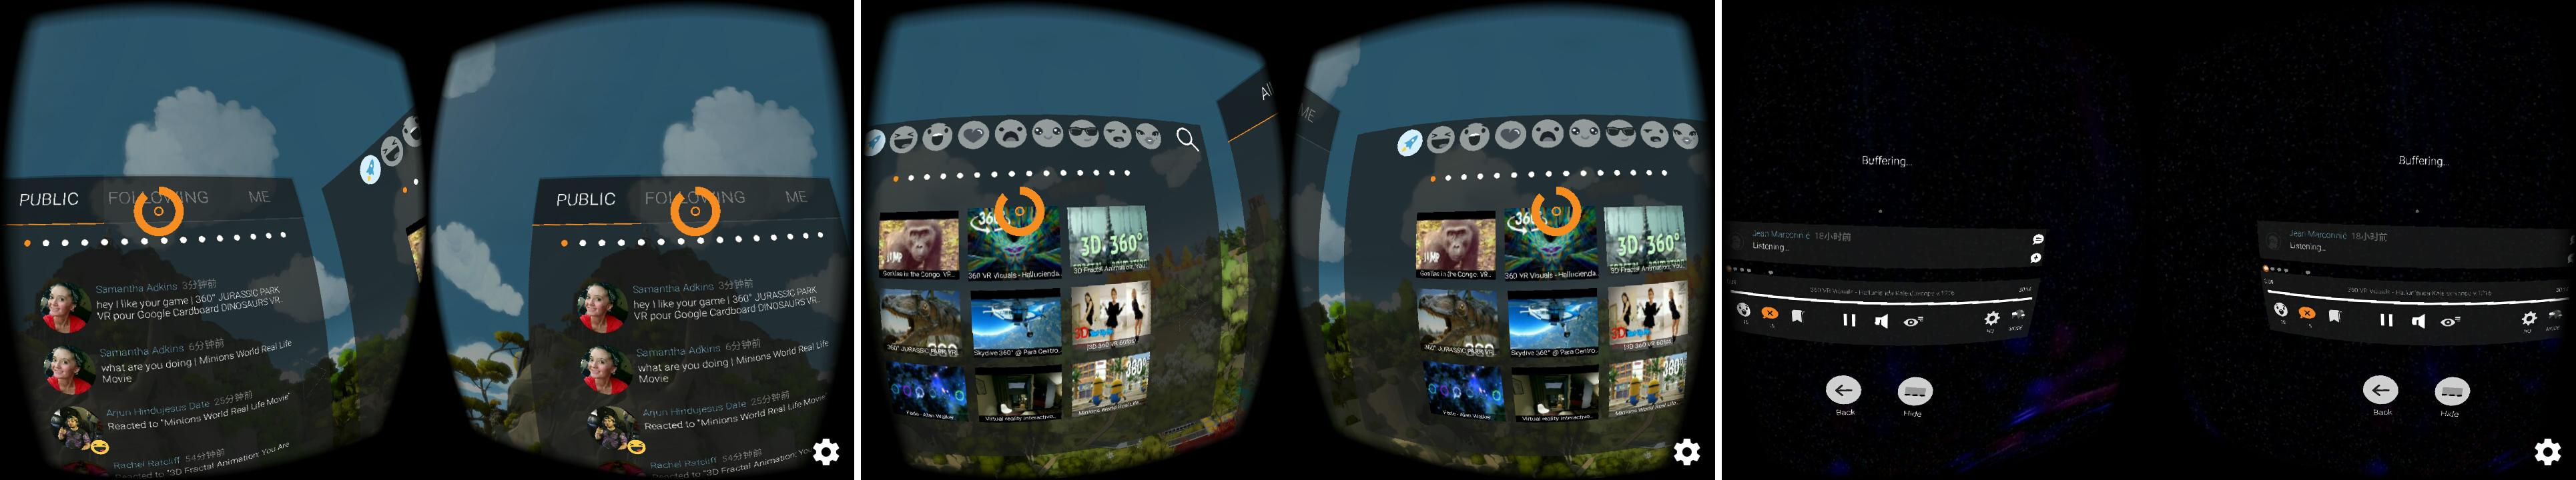
\includegraphics[width=.6\textwidth]{fulldive3}
}
\caption{Fulldive 视线停留模拟点击}
\label{fig:fulldive3}
\end{figure}

当然,这种模拟点击的操作只适用于”确认/取消“这种布尔判断的操作,用户需要输入大段的文字时则需有更高效的方式。Fulldive 结合了已日益成熟的语音识别技术,图\ref{fig:fulldive4}为实际操作 Fulldive 搜索功能并口述”中国地质大学“后的 APP 截屏。

\begin{figure}[htp]
\centering
\fbox{
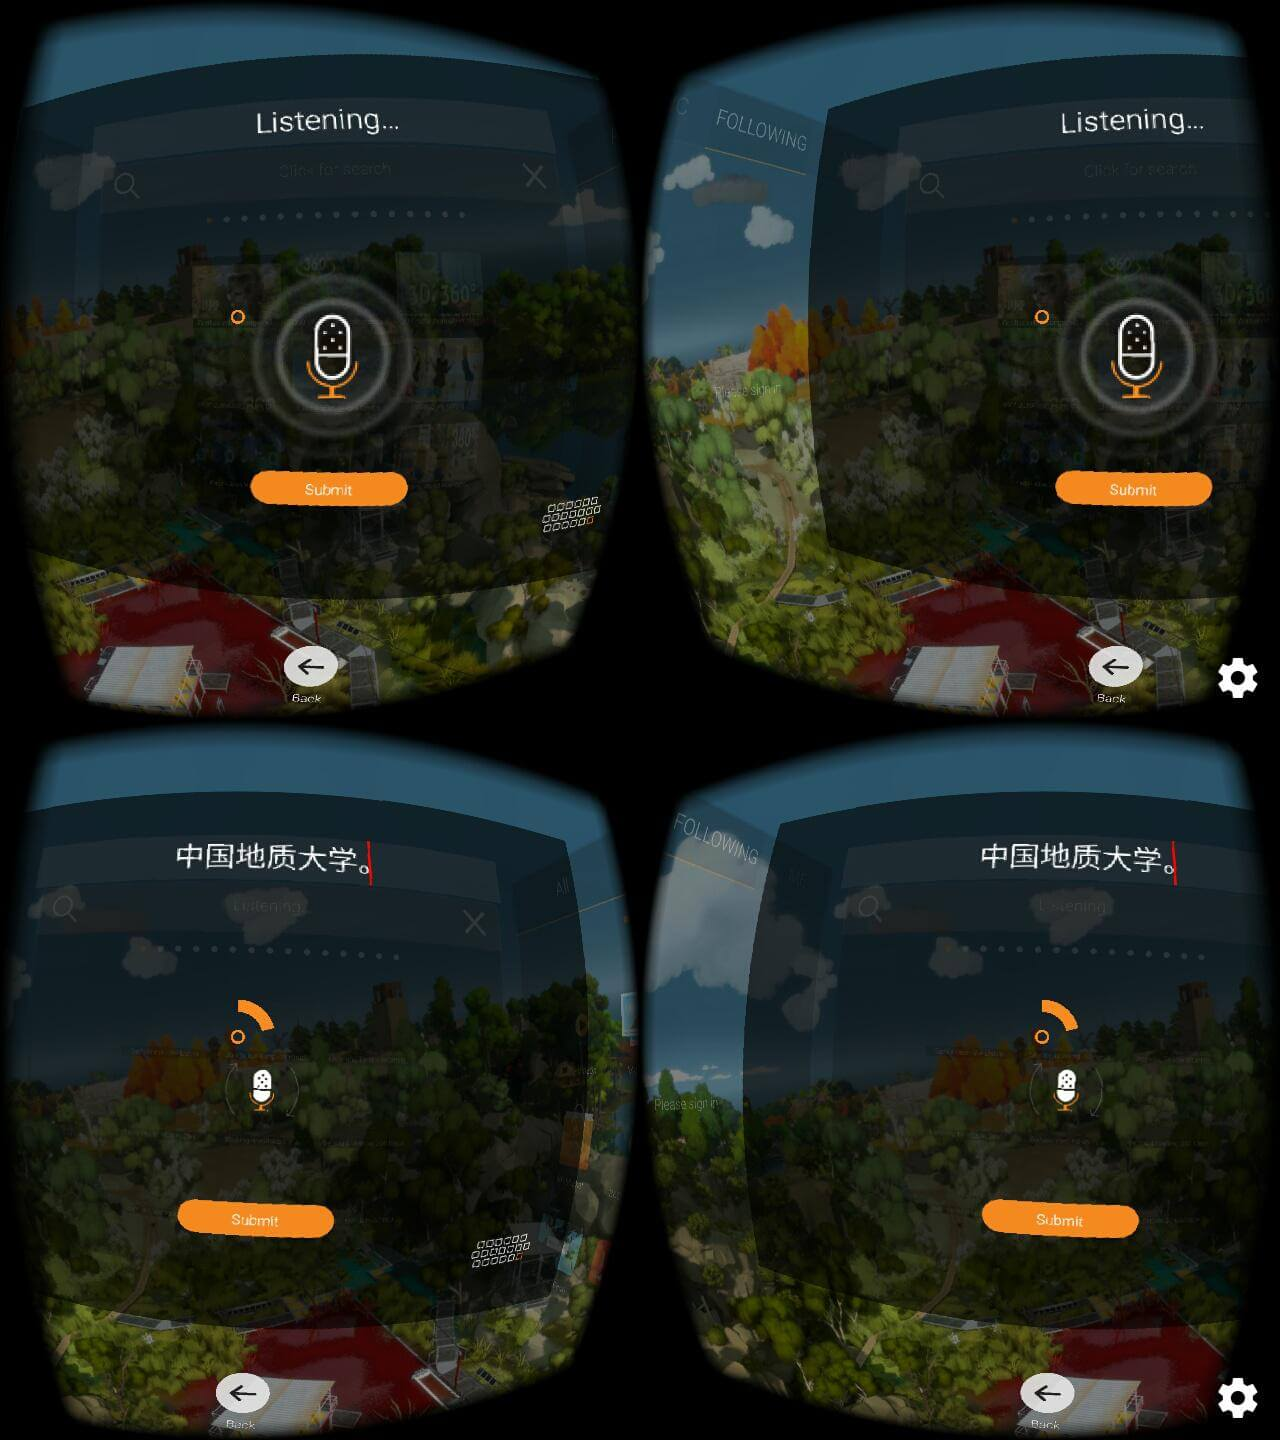
\includegraphics[width=.5\textwidth]{fulldive4}
}
\caption{Fulldive 语音识别}
\label{fig:fulldive4}
\end{figure}

\subsection{VR X-Racer}

VR X-Racer 是一款简单的 VR 操控类飞行游戏,其操作方式为晃动设备(如 VR 眼镜或手机)来控制屏幕上的飞机躲避障碍物,见图\ref{fig:x-racer}。这是全景漫游技术在游戏上最直接的体现:几乎没有多余的操作,在游戏中飞机撞到障碍物坠毁后若干秒即自动重新开始游戏。但其最大的缺陷是无法长时间使用,不断晃动的全景屏幕容易使人产生眩晕、恶心等不良反应。
全景漫游与 3D 影片的体验是完全不同的,全景漫游将用户完全包裹在视频所构建的封闭环境中,而 3D 眼镜只是对屏幕这种有限区域进行了折射。两者的区别在于 3D 影片由于有周围环境作为铺垫不易使人完全沉浸其中,全景漫游则是在很短的时间内(20-30 秒)就使人沉浸在虚拟世界中,直至摘掉全景设备重新适应周围环境。

\begin{figure}[htp]
\centering
\fbox{
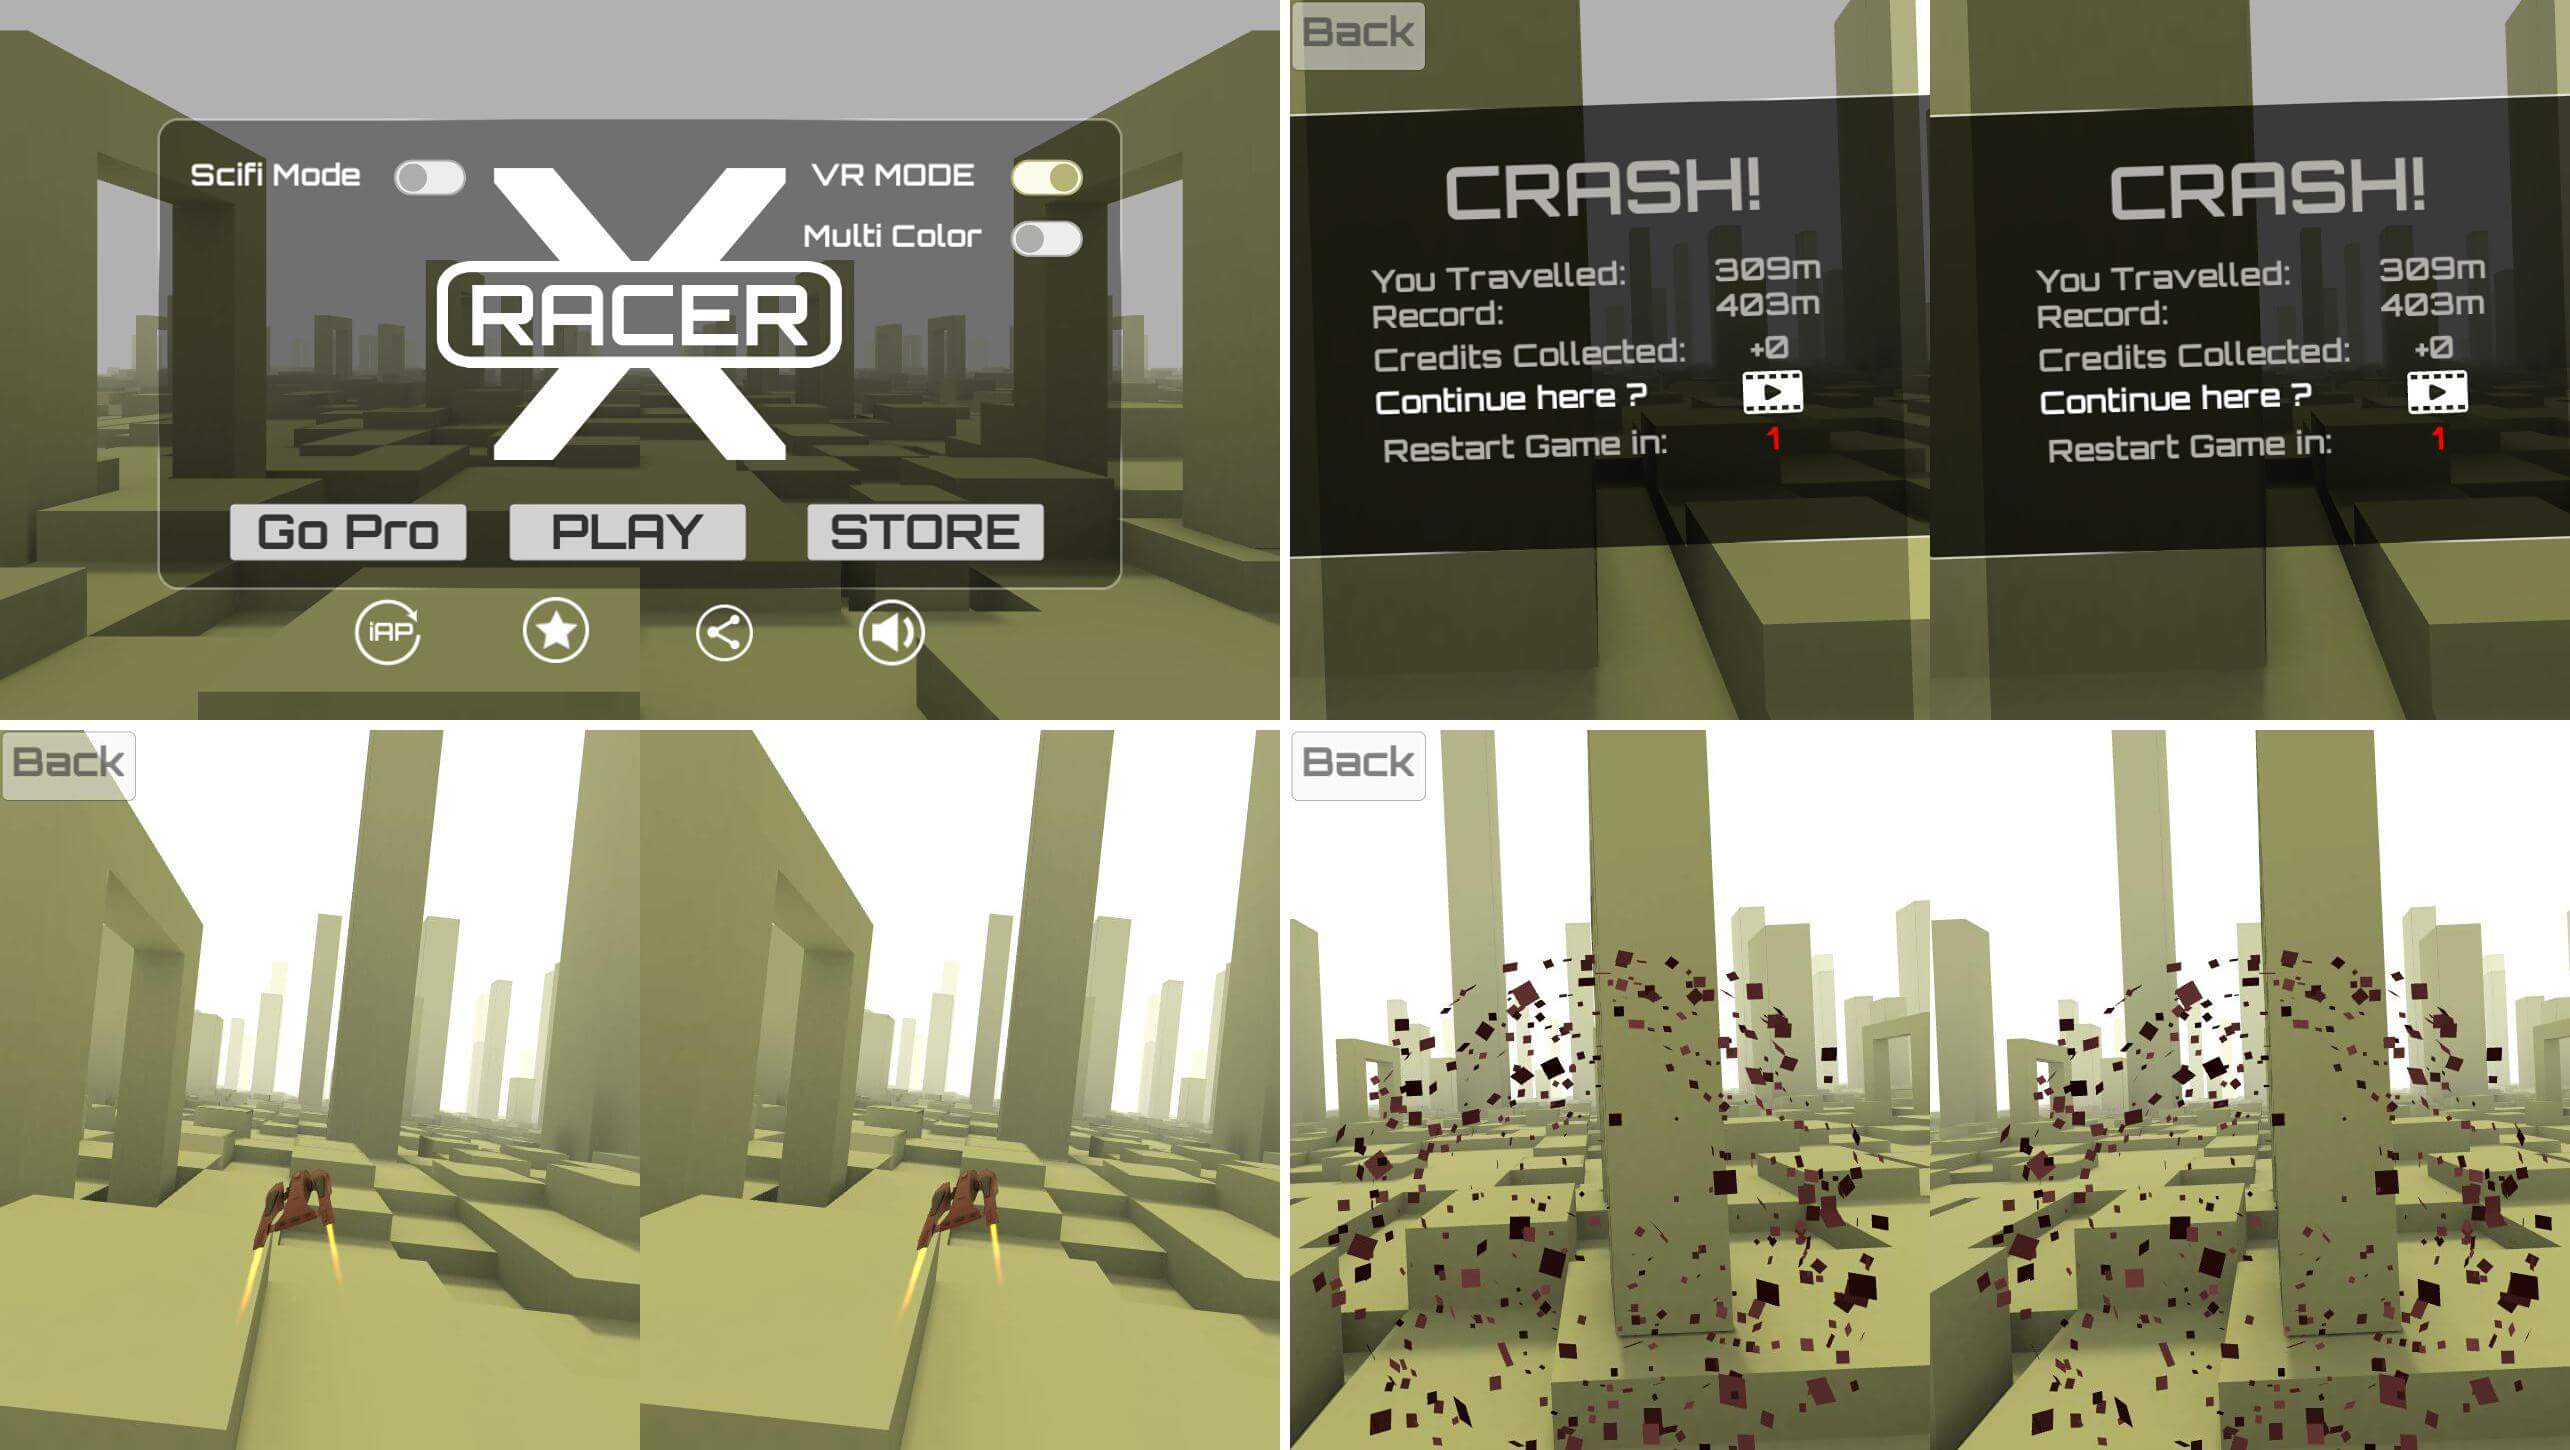
\includegraphics[width=.5\textwidth]{x-racer}
}
\caption{X-racer 游戏截图}
\label{fig:x-racer}
\end{figure}

\subsection{暴风魔镜 VR}

暴风影音是国内在全景漫游生态领域探索前沿的产品之一,其高端产品售价可达数千元,甚至与国外高端 VR 设备如 Oculus 和 GearVR 等价格相齐。与其硬件设备配套的则是一款叫做“暴风魔镜 VR”的手机 APP。

国内 APP 的发展方向一直是“大而全”,这款 APP 也不例外。暴风魔镜 VR 力图包括网络/本地视频、影音播放与 VR APP 等多种应用,形成自己的 VR 平台体系。同时支持普通的 APP 界面操作模式和全景漫游的 VR 模式。

在交互形式上与上文所列举的 Fulldive 类似,均为视线聚焦停留数秒视为确认,但缺少了语音识别输入大段文字的功能(在页面模式下支持手机输入法输入),如图\ref{fig:storm}。总体使用可满足基本的全景漫游体验,但识别速度较慢或误识别是比较严重的问题。

值得注意的一点是,暴风魔镜 VR APP 内场景下方有一个“归位”图标,触发后将会调整屏幕主视域至正对当前屏幕的位置,可类比于传统 APP 的“回到顶部”功能。这个功能很方便地起到了定位自身的作用,让用户不必盲目转动来寻找起始时正对着的界面。


\begin{figure}[htp]
\centering
\fbox{
  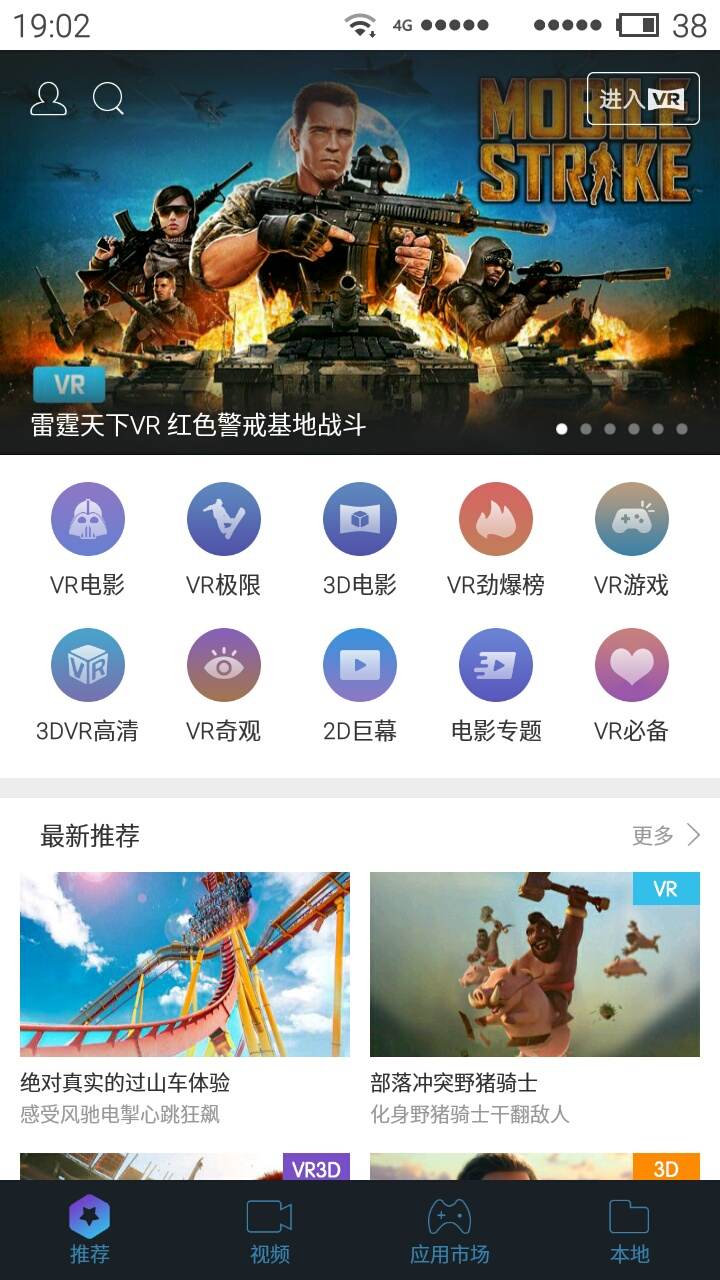
\includegraphics[width=.22\textwidth]{storm1}
}
\fbox{
  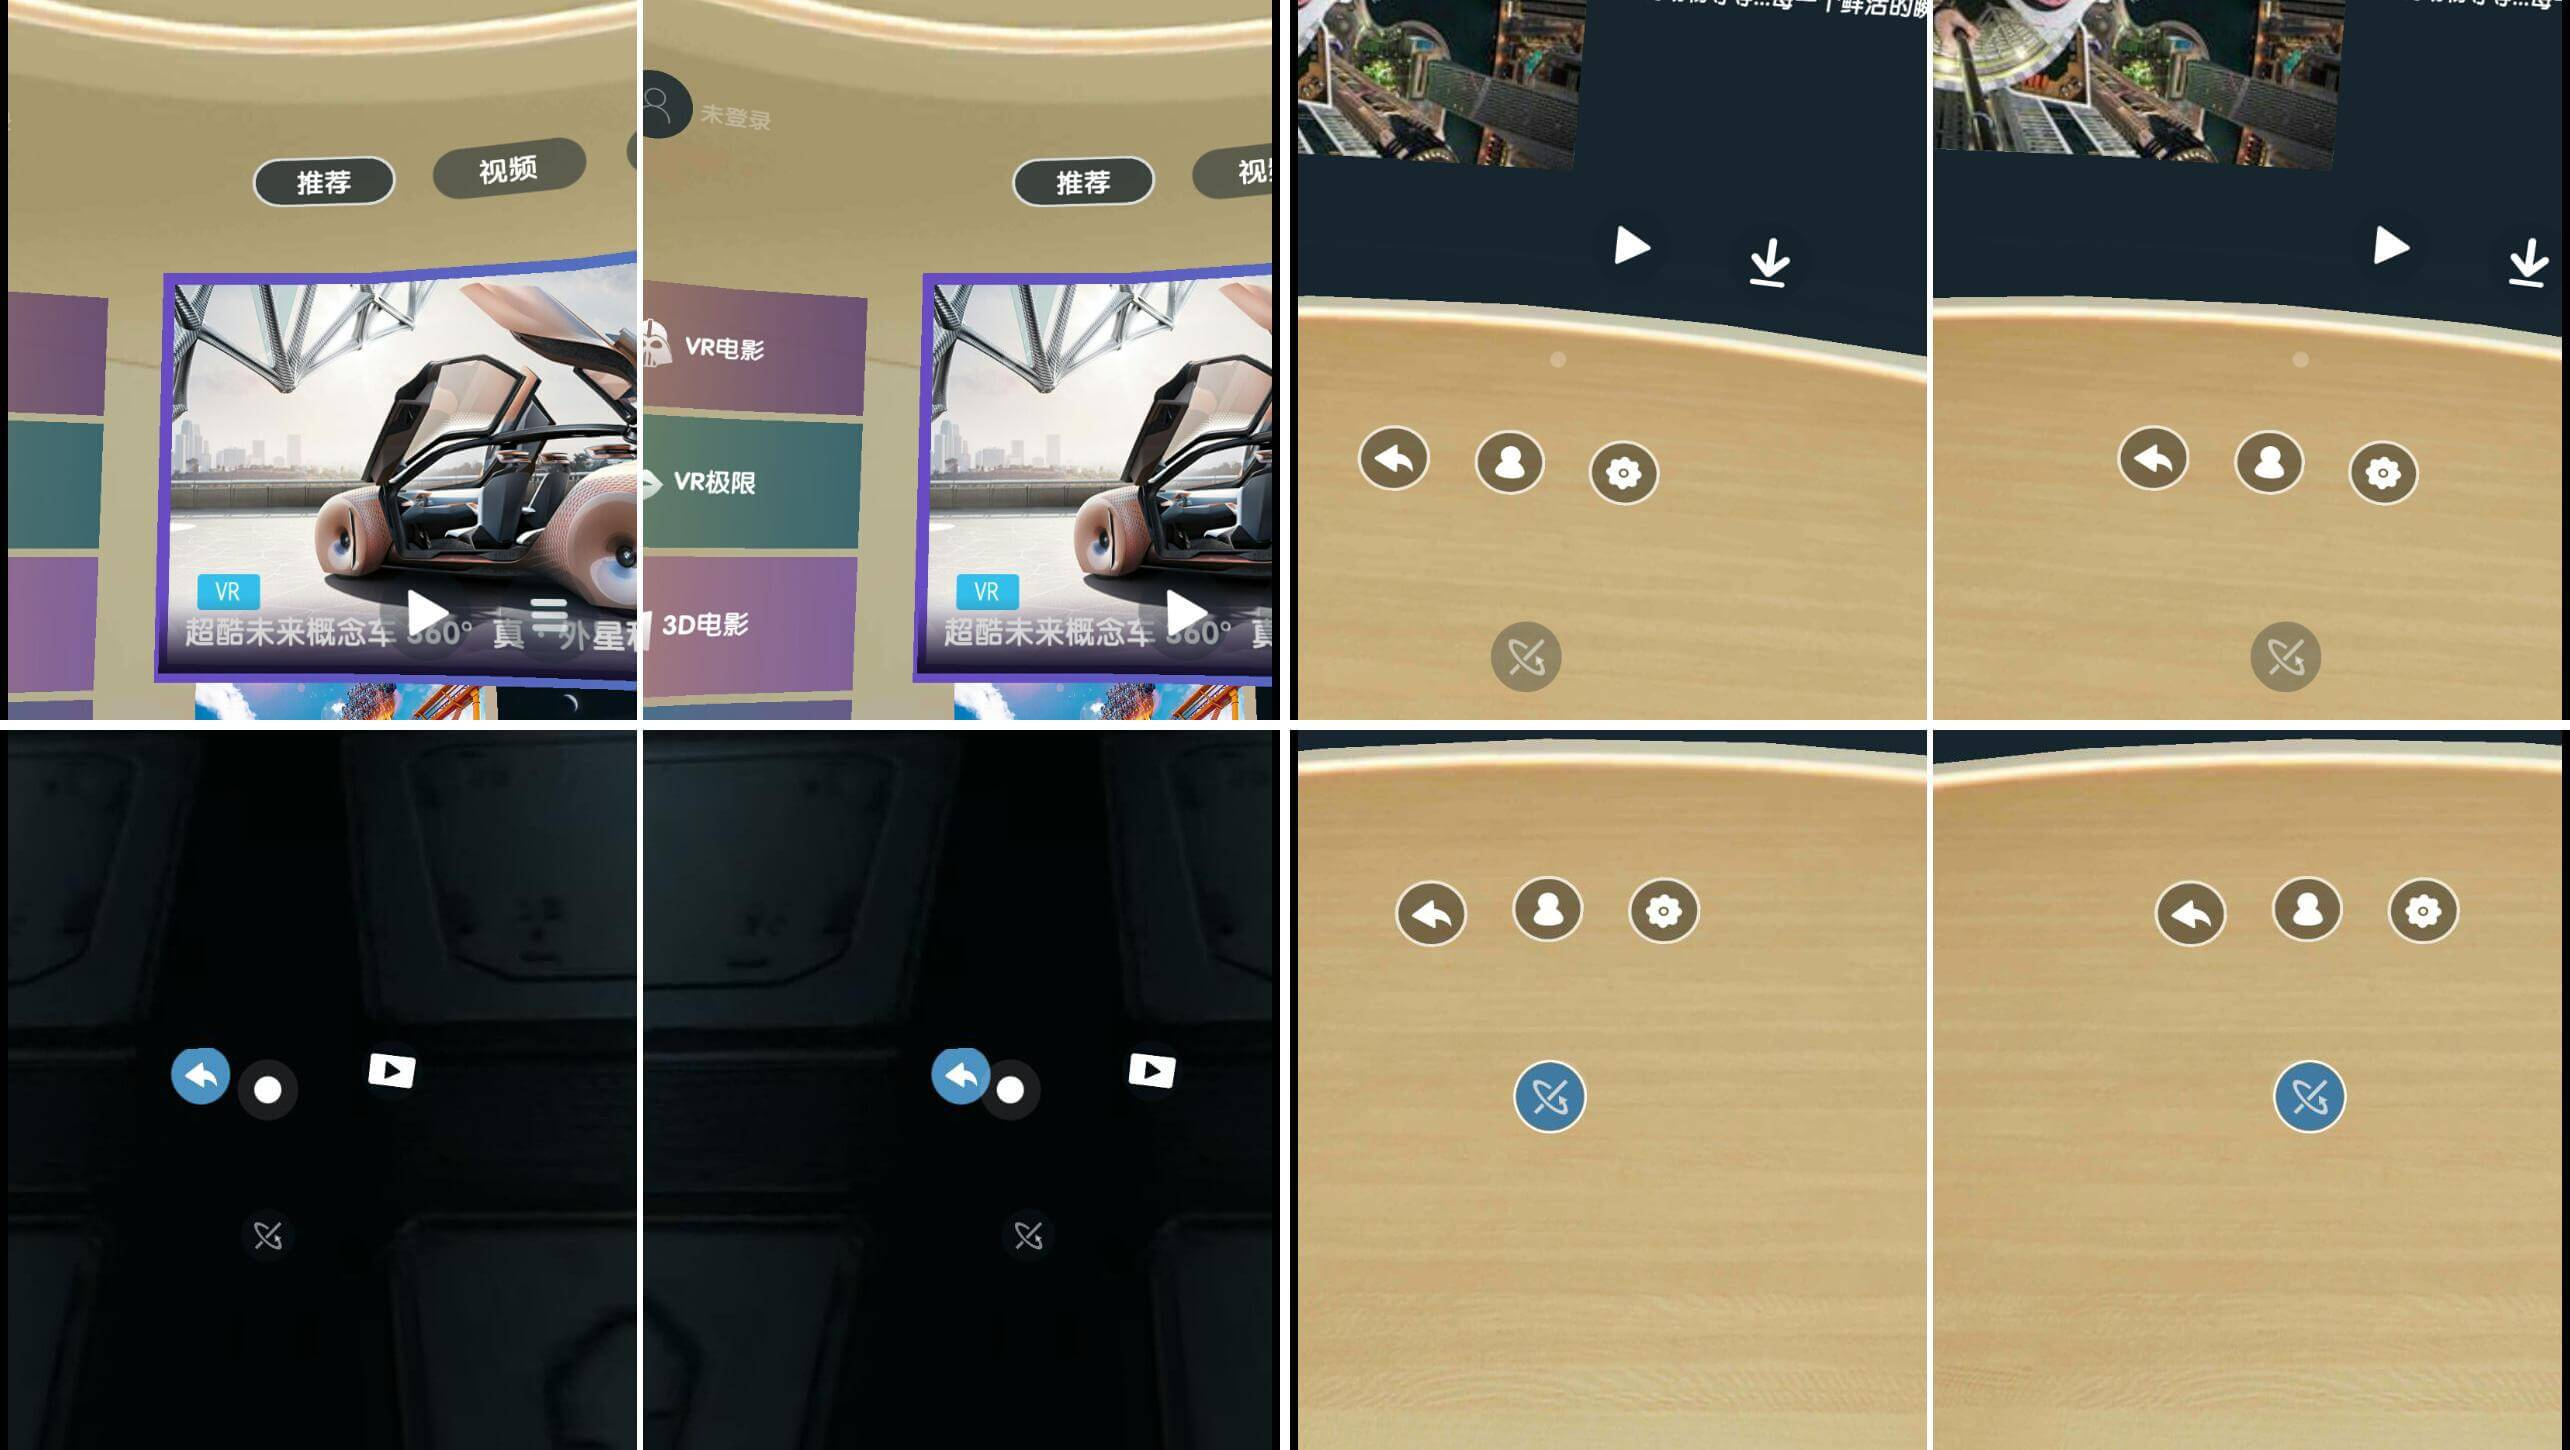
\includegraphics[width=.68\textwidth]{storm2}
}
\caption{暴风魔镜 VR 操作方式}
\label{fig:storm}
\end{figure}
